\subsection{Directional Lights}

\begin{frame}{Directional Lights - The Sun Model}
  \begin{columns}
    \begin{column}{0.6\textwidth}
      \begin{raybox}{Directional Light Concept}
        \small
        Light source at infinite distance, so rays are effectively parallel

        \only<2>{
          \vspace{0.3cm}
          \textbf{Characteristics:}
          \begin{itemize}
            \item Parallel rays
            \item Same intensity everywhere
            \item No attenuation
            \item Defined by direction only
          \end{itemize}
        }

        \only<3->{
          \vspace{0.3cm}
          \textbf{Perfect for:} Sun, moon, distant lights
        }
      \end{raybox}

      \only<4->{
        \begin{center}
          \begin{figure}
            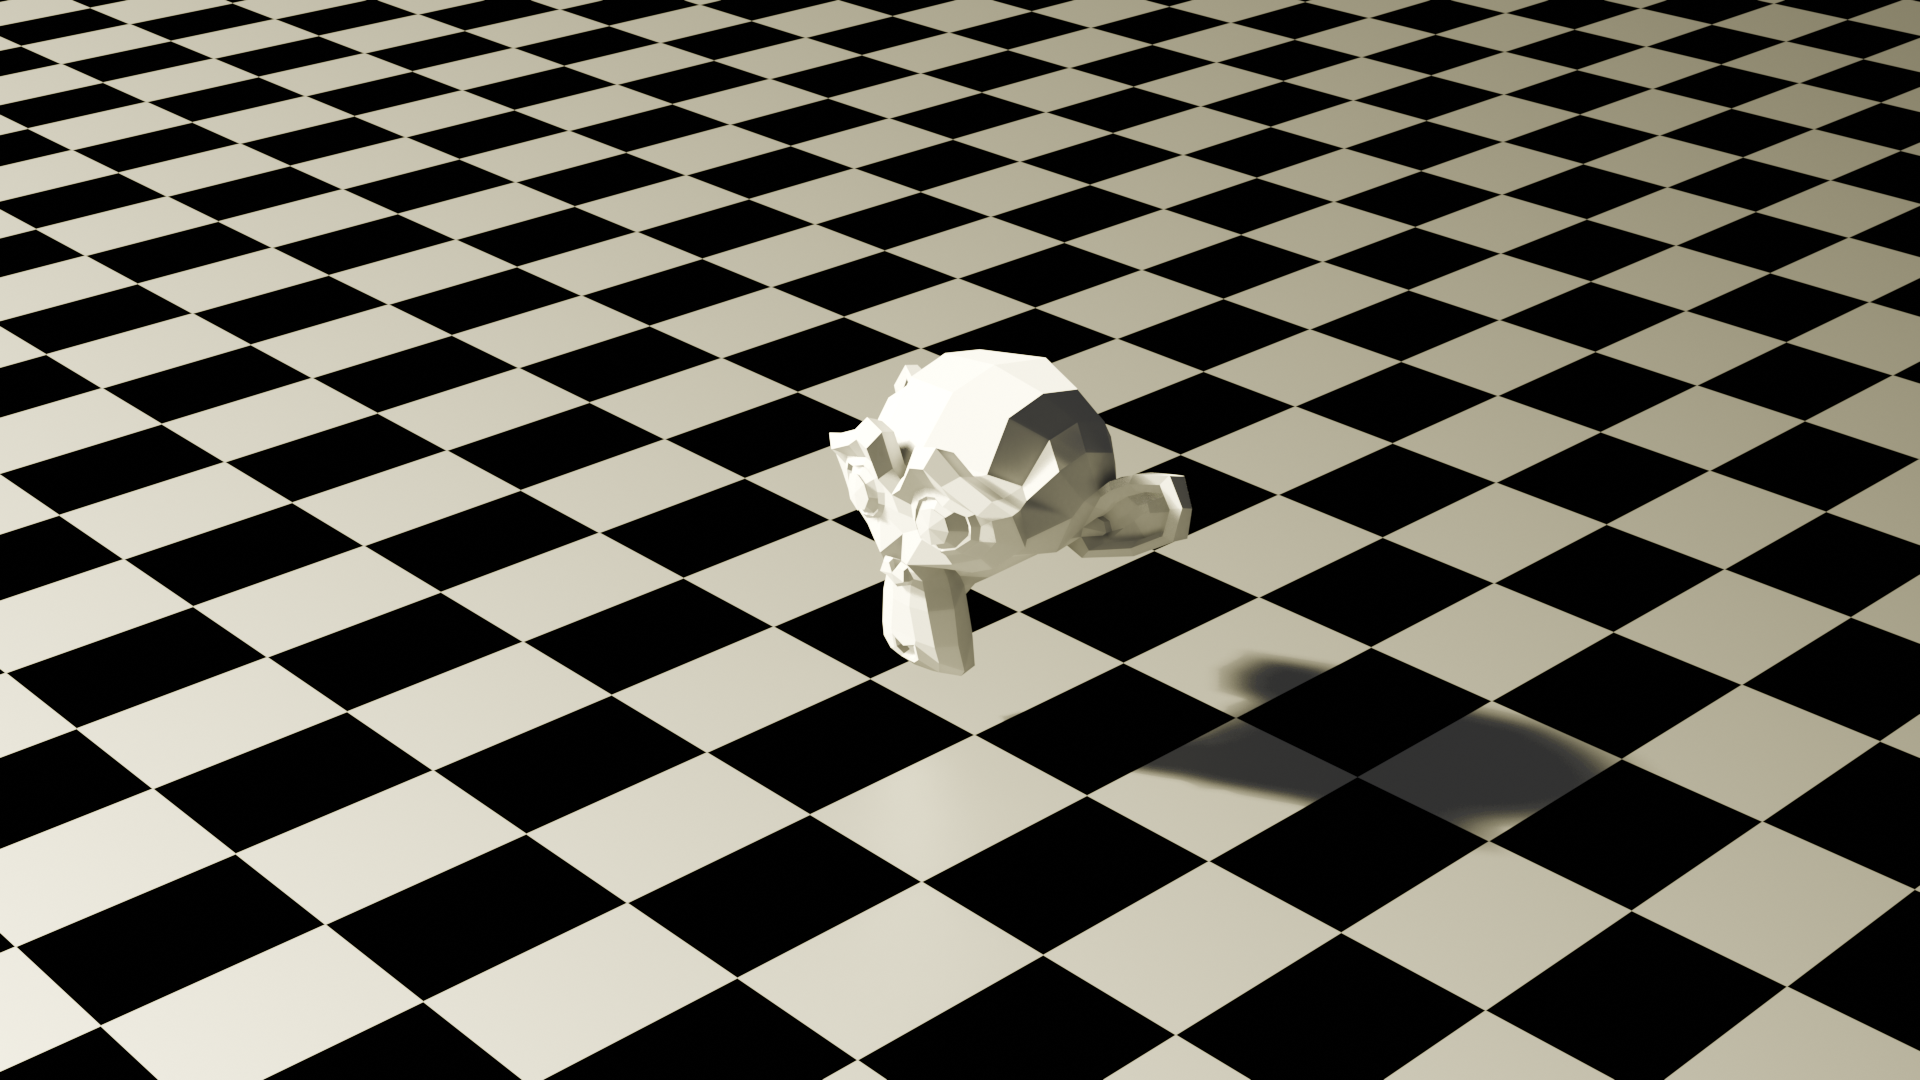
\includegraphics[width=\linewidth]{images/dir.png}
            \caption*{Directional Light ft. Suzanne}
          \end{figure}
        \end{center}
      }
    \end{column}
    \begin{column}{0.4\textwidth}
      \centering
      \scriptsize
      \begin{tikzpicture}[scale=0.5]
        % Sun (very far away)
        \node[circle, fill=LightColor, minimum size=1cm] (sun) at (-3,2) {\faIcon{sun}};
        \node[above] at (-3,2.7) {\footnotesize Sun (very far)};

        % Parallel rays
        \foreach \y in {0.5,1,1.5,2,2.5,3,3.5} {
          \draw[lightray, ->, thick] (-1,\y) -- (3.5,\y);
        }

        % Objects receiving parallel light
        \node[sphere, minimum size=0.8cm] (obj1) at (1,1) {};
        \node[sphere, minimum size=0.8cm] (obj2) at (3,3.5) {};

        % Direction vector
        \draw[->, red, very thick] (0,-2) -- (1.5,-2);
        \node[below] at (0.75,-2.3) {\footnotesize $\mathbf{L}$ (same for all points)};

        % Equal intensity indication
        \node[below] at (1,0.3) {\footnotesize Same intensity};
        \node[below] at (3,5) {\footnotesize Same intensity};
      \end{tikzpicture}
    \end{column}
  \end{columns}

\end{frame}

\begin{frame}{Directional Light Mathematics}
  \begin{columns}
    \begin{column}{0.6\textwidth}
      \begin{mathbox}{Directional Light Parameters}
        \textbf{Direction:} $\mathbf{D}_l = (x, y, z)$

        \textbf{Intensity:} $\mathbf{I}_l$ (constant)
        \vspace{0.3cm}
        \only<2->{
          \textbf{Light direction:}
          \begin{align*}
            \hat{\mathbf{L}} = -\mathbf{D}_l
          \end{align*}
          \only<2>{
            \footnotesize
            \textbf{Note:} Assuming $\mathbf{D}_l$ is normalized
          }
        }

        \only<3->{
          \textbf{Intensity at any point:}
          \begin{align*}
            I_{\text{final}} = \mathbf{I}_l \quad \text{(no attenuation)}
          \end{align*}
        }
      \end{mathbox}
    \end{column}
    \begin{column}{0.4\textwidth}
      \begin{tikzpicture}[scale=0.8]
        \begin{scope}[plane origin={(2,1,0)},
            plane x={(1.293,1.707,0)},
            plane y={(2,1,1)},
          canvas is plane]
          \draw[ObjectColor, fill=ObjectColor!20, opacity=0.6] (0,0) circle (2);
        \end{scope}

        \node[circle, fill=LightColor, minimum size=1cm] (sun) at (2,6) {\faIcon{sun}};

        \foreach \x in {0.5,1,1.5,2,2.5,3,3.5} {
          \draw[lightray, ->, thick] (\x, 5) -- (\x,4);
        }

        % Direction vector from light
        \draw[->, lightray, very thick] (2,3) -- (2,1);
        \node[right] at (2.2,2) {\footnotesize  $\hat{\mathbf{L}} = -\mathbf{D}_l$};
        \node[above] at (2,3.3) {\footnotesize Light direction $\mathbf{D}_l$};

        % Surface point
        \fill[ObjectColor] (2,1) circle (3pt);
        \node[below] at (2,0.7) {\footnotesize Surface point};
        \draw[->, very thick, red] (2,1) -- (2,3);

      \end{tikzpicture}
    \end{column}
  \end{columns}
\end{frame}